% Two-column-width variant. Use figure, width=\columnwidth, and the
% *_column.pdf filename for a single-column version.
\begin{figure*}[t]
    \centering
    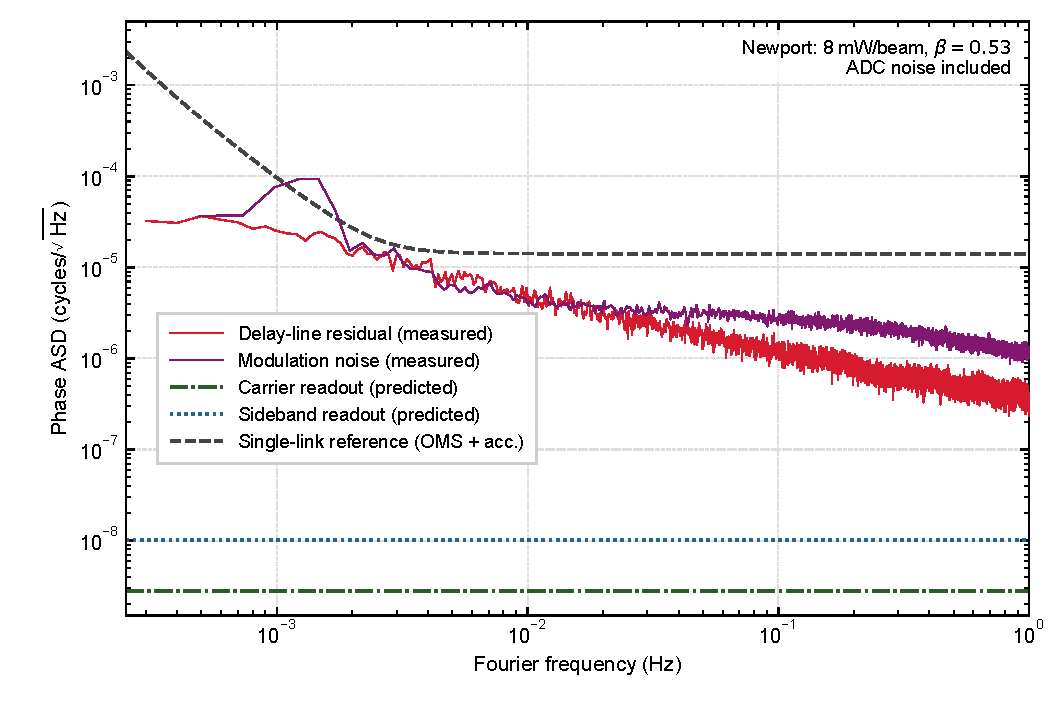
\includegraphics[width=\textwidth]{images/performance/component_inputs_single_link.pdf}
    \caption{Component phase-noise amplitude spectral densities compared with
    the single-link reference formed from optical metrology and acceleration
    noise. Solid curves show the measured delay-line residual and modulation
    phase-noise estimator; measured Fourier bins are plotted without smoothing.
    The illustrative linear-receiver carrier and first-order sideband readout noises
    include shot noise, dark-current shot noise, Johnson noise, relative
    intensity noise and ADC quantization noise. The optical model assumes one
    phase-modulated beam and one unmodulated reference beam, each delivering
    $4\,\mathrm{mW}$ at the detector, with modulation depth $0.53\,\mathrm{rad}$.
    The detector responsivity is $0.6\,\mathrm{A/W}$, heterodyne efficiency is
    $0.9$, and the termination is $50\,\Omega$ at $300\,\mathrm{K}$.
    The ADC model uses a $1\,\mathrm{V}$ full-scale span, 14 bits and
    $2\,\mathrm{GS/s}$, with an ideal three-way electrical split. The assumed white RIN is
    $0.9\times10^{-8}/\sqrt{\mathrm{Hz}}$, summed coherently between the beams.
    The model uses $(35,36,34)\,\mathrm{MHz}$ modulation and electrical carrier
    frequencies of $15.0$, $10.9$ and $21.6\,\mathrm{MHz}$; the readout
    prediction assumes white noise across the corresponding RF bands.
    All curves are shown before propagation through TDI and clock correction;
    the measured electronic residual is shown as characterized and is not
    deconvolved into individual board noise sources. The assumptions of the component budget are stated in Section~\ref{sec:performance}. }
    \label{fig:component_inputs_single_link}
\end{figure*}
